\section{Results}
\label{sec6}
In this section, we compare the bounds obtained via our novel method to bounds obtained using the transfer function method as well as the simulation results for three RSC codes. For each RSC code and a frame size of $N=64$, the codeword is BPSK modulated and transmitted over the AWGN channel. At the receiver end, the Viterbi algorithm is used to decode before a decision is made on the decoded sequence.

\begin{figure}[h!]
\centering
		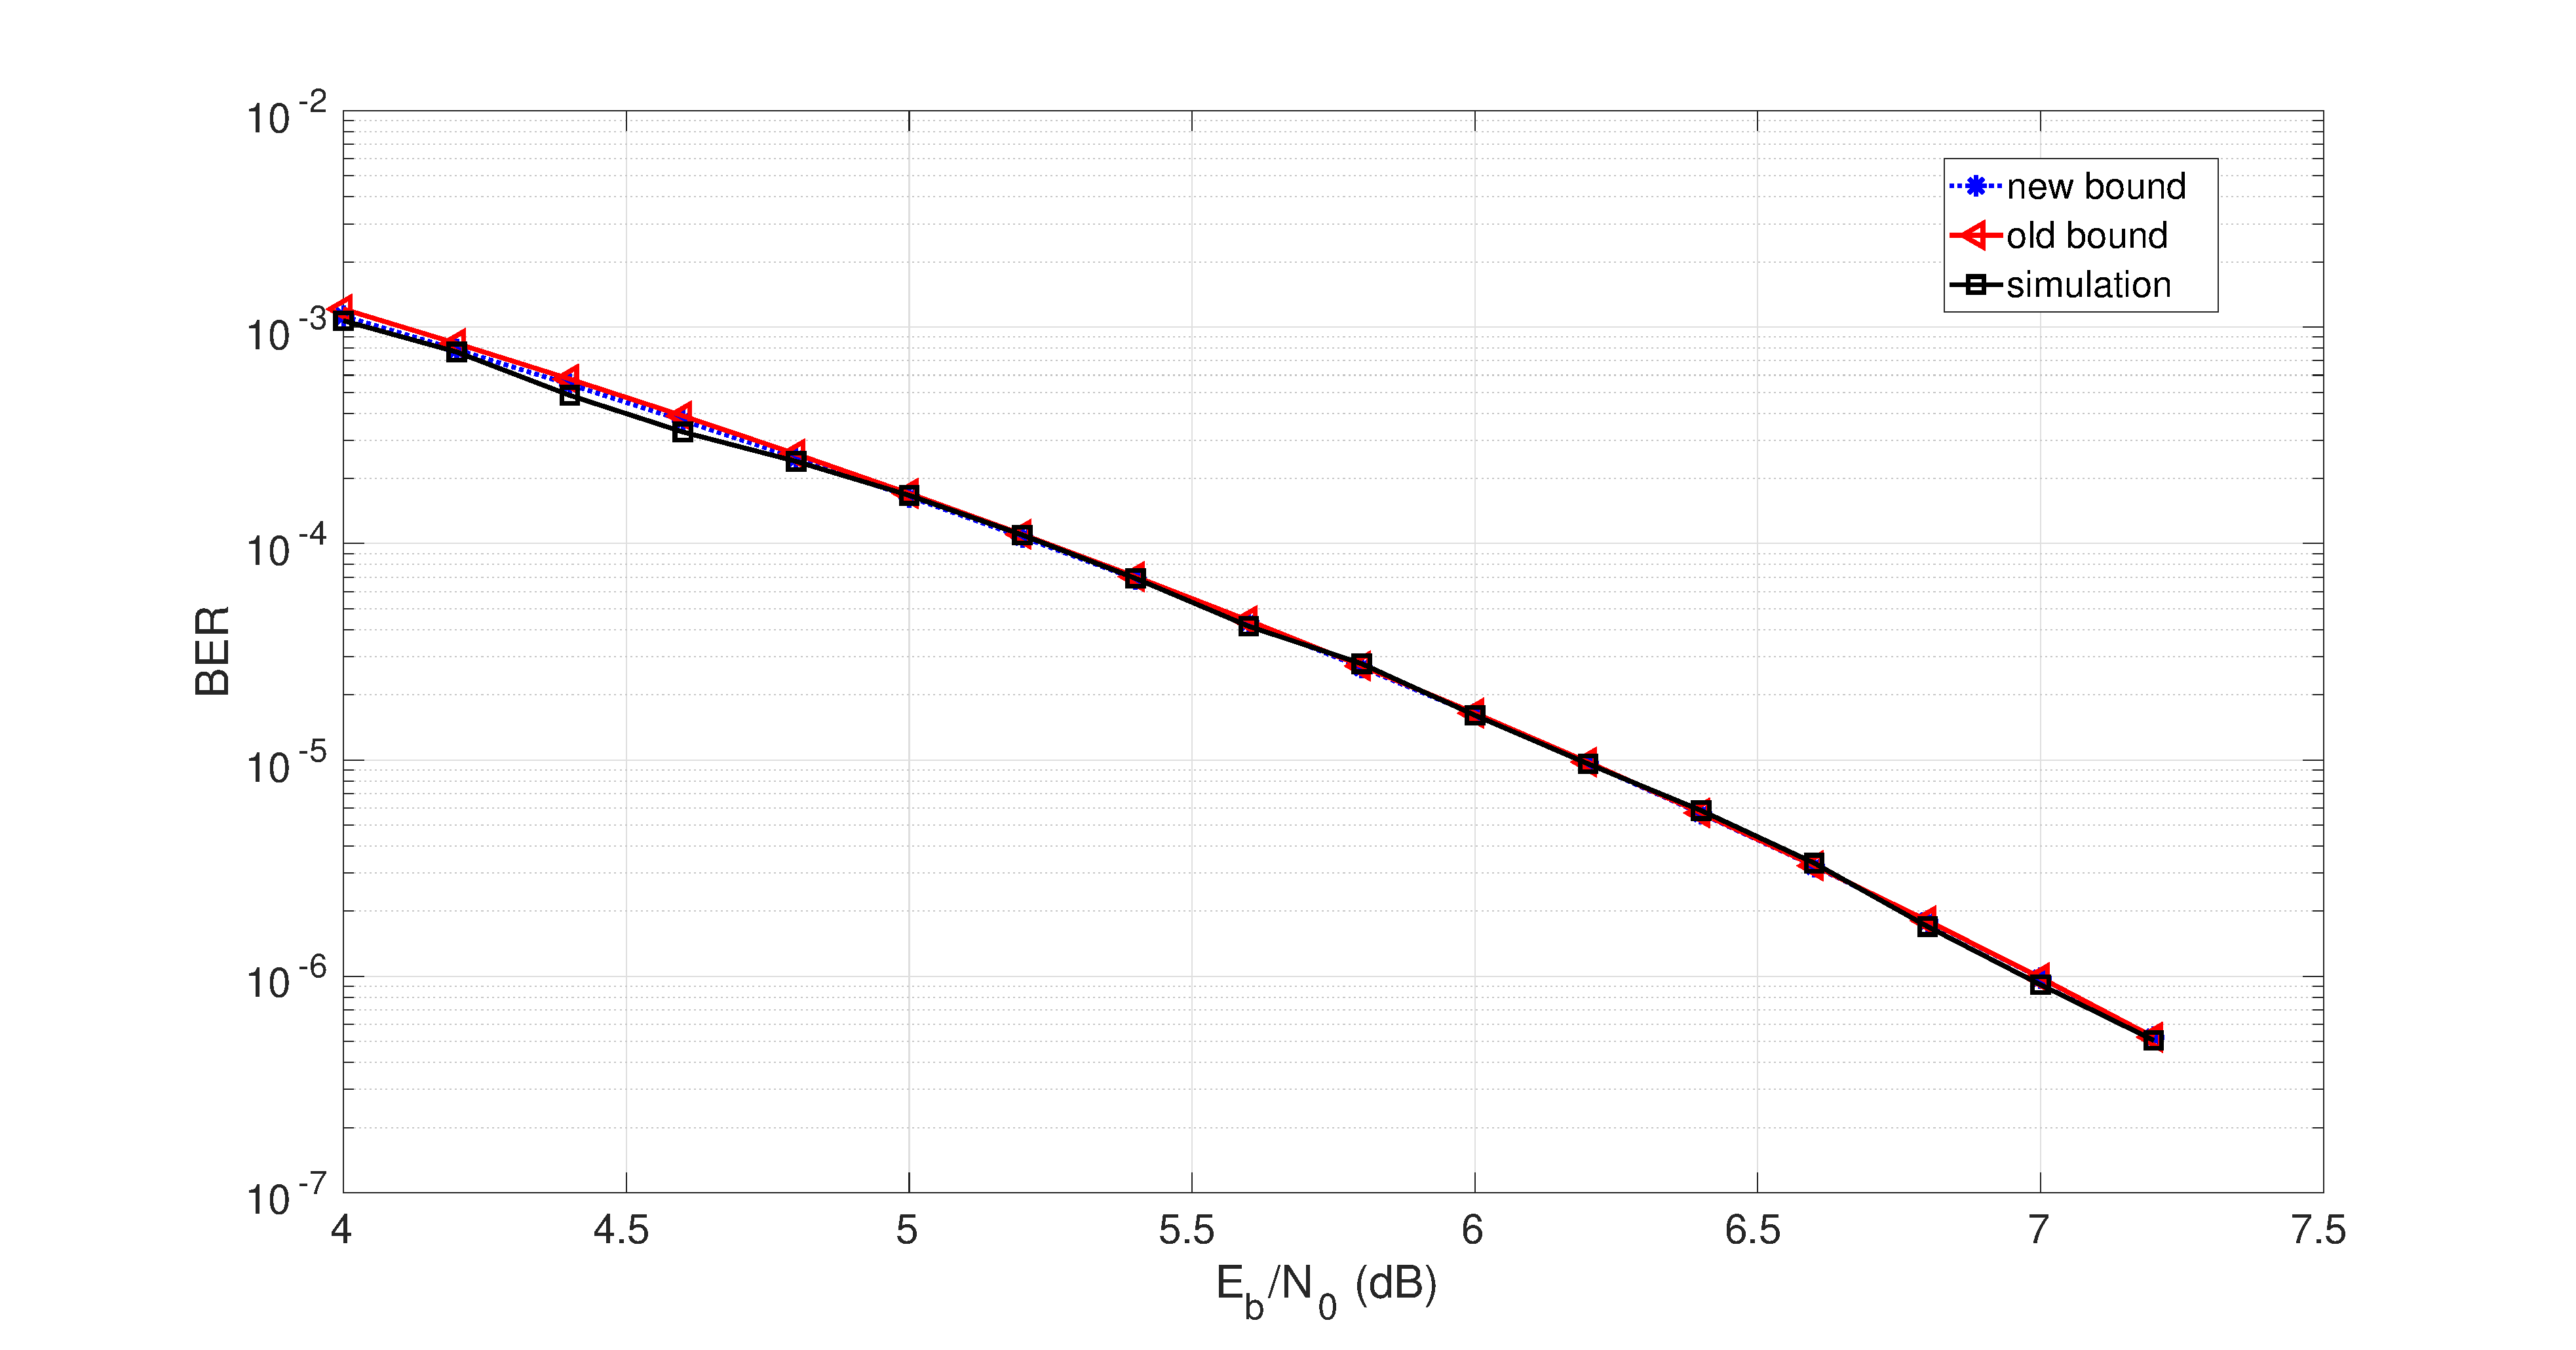
\includegraphics[width=0.5\textwidth]{./Images/RSC_5_7_lower_weights.eps}
		\caption{Old Bound vs New Bound vs Simulation for 5/7 RSC Code}
		\label{simFig1}
		\end{figure}
We observe that for both Fig. \ref{simFig1} and Fig. \ref{simFig2}, there is some difference between the new (novel method) bound and the old (transfer function) bound, but they tend to converge as $E_b/N_0$ increases. This suggests that codewords generated considering $b(x),~w_H(\bb)>3$ as well as codewords which have a parity-check sequence $h(x),~w_H(\bh)>3$ do not have much effect on the BER of the code as $E_b/N_0$ increases.

%The gap that is observed in the low $E_b/N_0$ regions is attributed to omitting codewords generated by the RTZ inputs of weight $w_H(\bb)=4$ as well as codewords with parity-check sequences $w_H(\bh)=4$ in our calculation of the new bound. 

%Fig. \ref{simFig4} and Fig. \ref{simFig5} are similar to  Fig. \ref{simFig1} and Fig. \ref{simFig2}, with the only difference being that codewords generated by the RTZ inputs of weight $w_H(\bb)=4$ as well as codewords with parity-check sequences $w_H(\bh)=4$ have been added in our calculation of the new bound. The new and old bounds match up and the accuracy of our bound is greatly improved.The simulation results also agree with the bounds as they also converge with the bounds.
\begin{figure}[h!]
\centering
		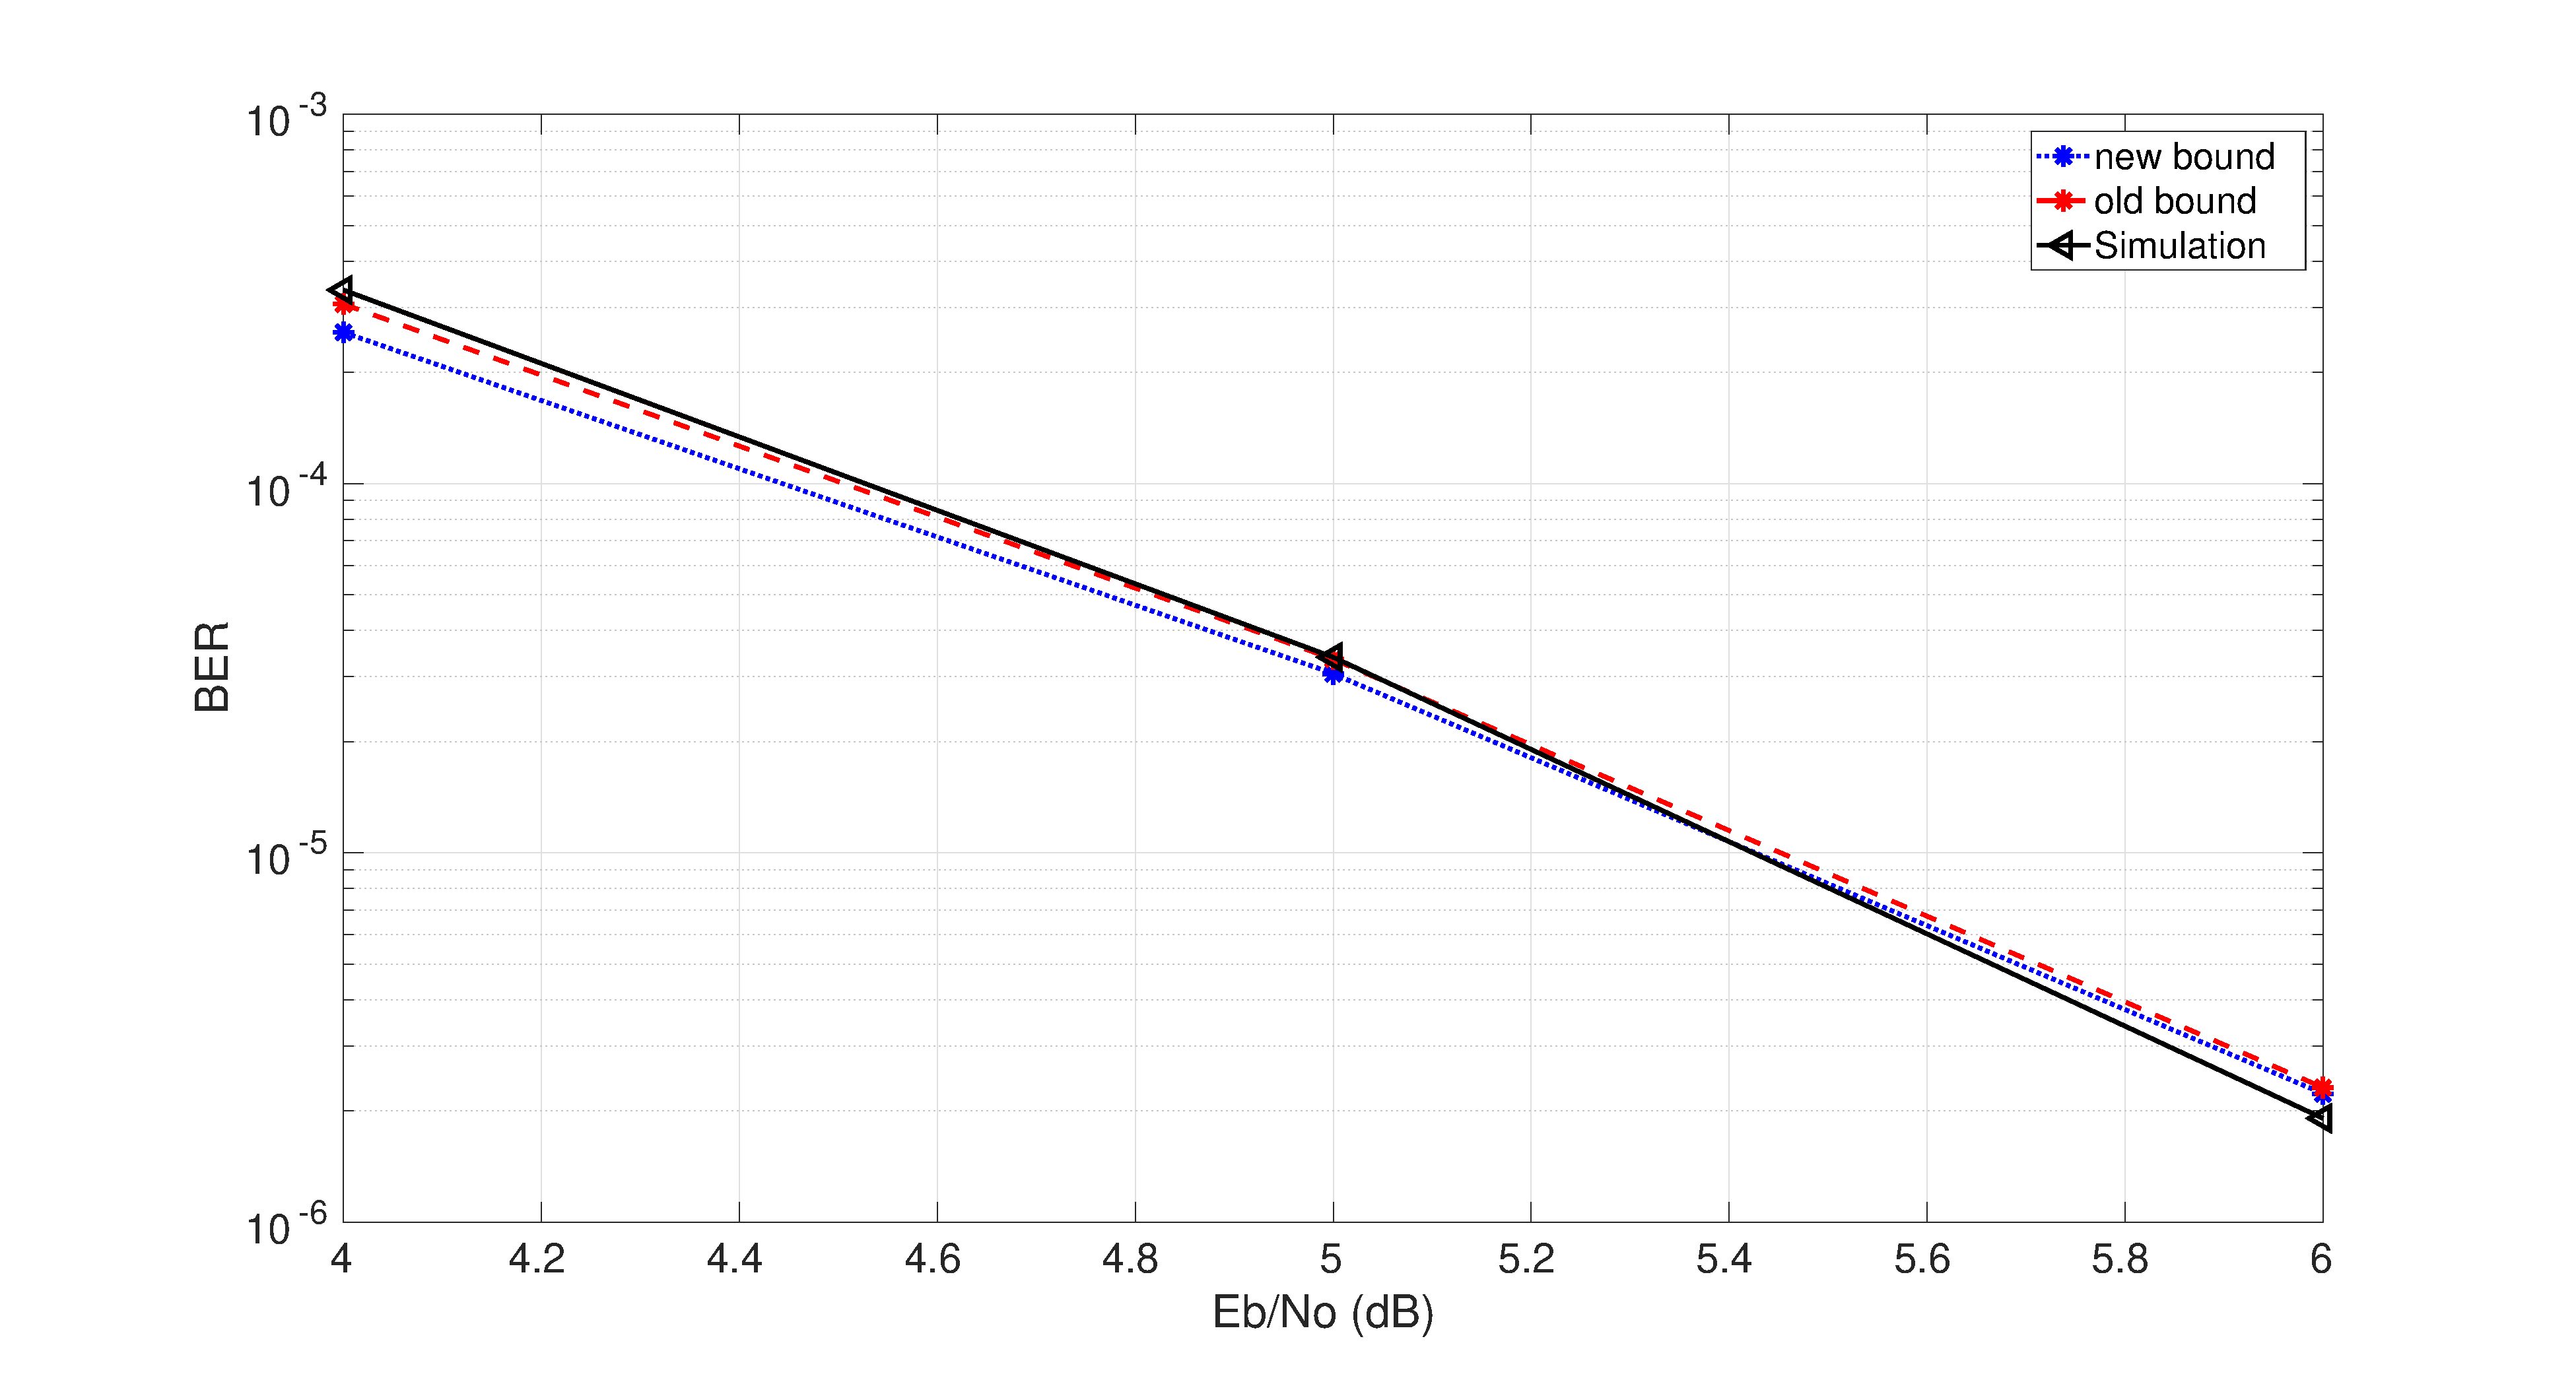
\includegraphics[width=0.5\textwidth]{./Images/RSC_37_21_v2.eps}
		\caption{Old Bound vs New Bound vs Simulation for 37/21 RSC Code}
		\label{simFig2}
		\end{figure}
However, in Fig. \ref{simFig3}, it is apparent that codewords generated by higher weight RTZs as well as those with parity-check sequences with weights $w_H(\bh)>3$ still dominate at higher $E_b/N_0$ values and need to be considered. As can be observed from the graph, there is a very distinct gap between the new bound and the old bound. Moreover, the bounds do not converge as $E_b/N_0$ increases. However, the old bounds and simulation results converge as the $E_b/N_0$ value increases. 
%In \ref{simFig3}, we observe that the old bounds and simulation results converge as the Eb/No value increases. However, there is a very distinct gap between the new bound and the old bound. Moreover, the bounds do not converge as the Eb/No increases. This means that we are missing vital elements in our approximation by not considering codewords generated by RTZ inputs of weight $w_H(\bb)>3$ as well as codewords with parity-check sequences $w_H(\bh)>3$. 

\begin{figure}[h!]
\centering
		\includegraphics[width=0.5\textwidth]{./Images/RSC_23_35_v3.jpg}
		\caption{Old Bound vs New Bound vs Simulation for 23/35 RSC Code}
		\label{simFig3}
		\end{figure}
		

%\begin{figure}[h!]
%\centering
%		\includegraphics[width=0.8\textwidth]{./Images/RSC_5_7_higher_weights.eps}
%		\caption{Old Bound vs New Bound vs Simulation for 5/7 RSC Code, with higher weights }
%		\label{simFig4}
%		\end{figure}
		
		
%		\begin{figure}[h!]
%\centering
	%	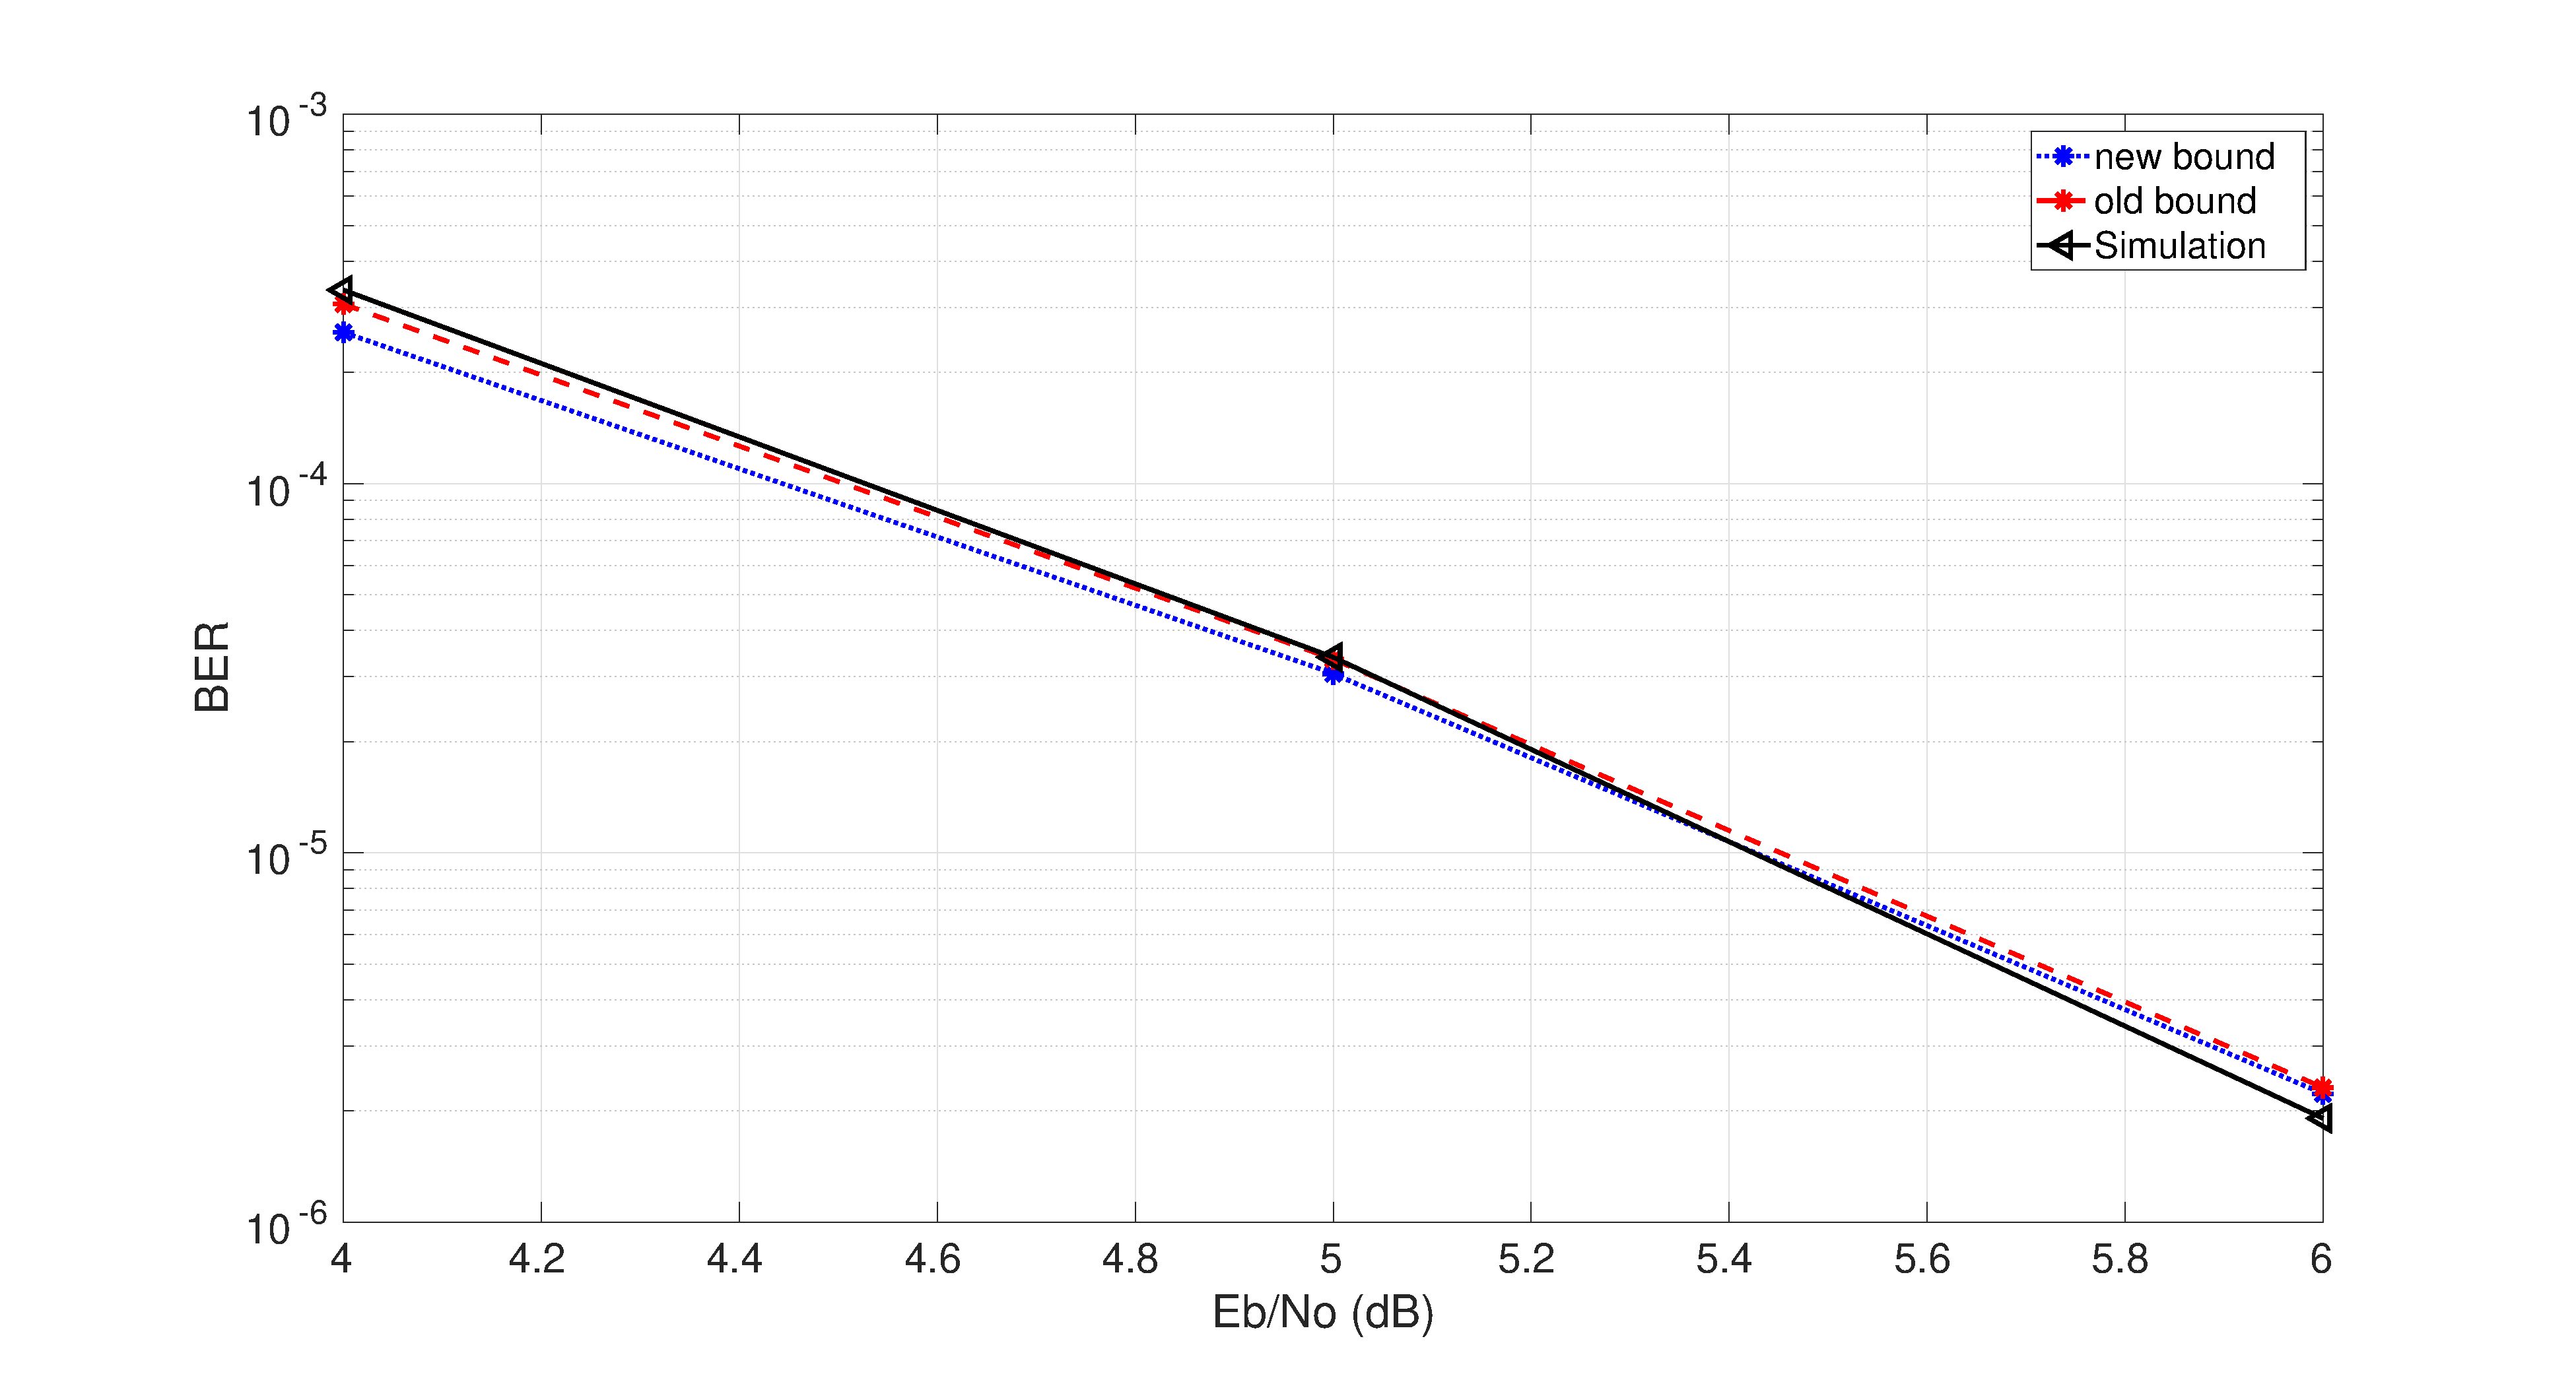
\includegraphics[width=0.5\textwidth]{./Images/RSC_37_21_v2.eps}
		%\caption{Old Bound vs New Bound vs Simulation for 37/21 RSC Code, with higher weights}
		%\label{simFig5}
		%\end{figure}


